\documentclass[11pt]{report}
\usepackage[backend=bibtex,style=numeric]{biblatex}
\usepackage[utf8]{inputenc}
\usepackage[english]{babel}
\usepackage[margin=1in]{geometry}
\usepackage[section]{placeins}
\usepackage{csquotes}
\usepackage{titlesec}
\usepackage[acronym]{glossaries}
\usepackage{mathtools}
\usepackage{minted}

\newcommand{\dd}[1]{\mathrm{d}#1}

\bibliography{references}

\title{\textbf{Calculus on Computational Graphs and Image Analysis}}
\author{
\begin{tabular}[t]{cc}
Champion Théophile \\
University of Kent \\
tmac2@kent.ac.uk \\
\end{tabular}
}
\date{\today}

\makeglossaries

\newglossaryentry{task_learning}
{
    name=Task learning,
    description={Task or supervised learning refer to the algorithms that aims to solve a task. In task learning, the expected output is known and part of the expected mapping is given to the models during the learning}
}
\newglossaryentry{model_learning}
{
    name=Model learning,
    description={Model or unsupersised learning refer to the algorithms that aims to create a model of the data. In model learning, the expected output is unknown and the models search for correlations, clusters or structures in the data}
}
 
\newacronym{cnn}{CNN}{Convolutional Neural Network}
\newacronym{conv_net}{ConvNet}{Convolutional Neural Network}
\newacronym{cpca}{CPCA}{Conditional Principal Component Analysis}
\newacronym{kwta}{kWTA}{k-Winners-Take-All}
\newacronym{hcnn}{HCNN}{Hebbian Convolutional Neural Network}
\newacronym{cpu}{CPU}{Central Processing Unit}
\newacronym{gpu}{GPU}{Graphics Processing Unit}
\newacronym{std}{STD}{Standard deviation}

\begin{document}

\maketitle

\tableofcontents

\glsaddall
\printglossary[type=\acronymtype, nonumberlist]
\addcontentsline{toc}{chapter}{Acronyms}
\printglossary[type=main, nonumberlist]
\addcontentsline{toc}{chapter}{Glossary}

\listoffigures
\addcontentsline{toc}{chapter}{List of Figures}
\listoftables
\addcontentsline{toc}{chapter}{List of Tables}

\newpage

\chapter{Introduction}

Image analysis is the field that aims to extract meaning from images. This is an important area of research in machine learning, which has found application from the reading of bar coded tags to the detection of cancerous tumors. It is needless to say that any improvement of the state-of-the-art will have an impact on a lot of domains. This thesis proprose new ideas to improve the convolutional neural network, which is the most popular model in the field.

\section{Objectives}

The first objectif of this paper is to propose a variation of the well known convolutional layer, which uses a mixture of task and model learning. This imply comparing the performance of this variation with the original convolutional layer in terms of computational time and accuracy.
\newline
\newline
\noindent The second aims of this paper is to implement it from scratch. This means recoding the graph logic of TensorFlow and being able to backpropagate the gradients through any non cyclic graph of computation. The flexibility provided by such logic will enable the implementation of state-out-the-art models used in computer vision.
\newline
\newline
\noindent The third goal of this project is to show how general purpose GPU programming can speed up neural networks. This will be done by comparing the CPU and the GPU implementation of various layers, such as max pooling and convolutional layers.

\section{Overview of Contents}

\paragraph{Chapter \ref{related_work}:} Present image analysis techiques as well as notions relevant to the chapter \ref{model_and_task_learning}.
\paragraph{Chapter \ref{model_and_task_learning}:} Propose a new model that learn from the structure of the data.
\paragraph{Chapter \ref{model_implementation}:} Dive into the implementation details of the model.
\paragraph{Chapter \ref{result_and_analysis}:} Analyse the model in terms of accuracy and learning speed.
\paragraph{Chapter \ref{framework_limitation}:} Explain the current limitation of the framework.
\paragraph{Chapter \ref{conclusion}:} Conclude the paper and propose future research directions.

\chapter{Realted Work} \label{related_work}

\section{Convolutional Neural Network}

The \acrshort{cnn} or \acrshort{conv_net} architecture \cite{NIPS1989_293} is a deep neural network learning by backpropagation. It is composed of two kind of layers: convoltion and pooling. The convolution layer contains kernels that will be slide through the image with step size defined by the strides. In recent implementation \cite{5537907} non-linear activation is added after the weighted sum produce by the kernels such as:
\begin{equation}
y_{convolution} = \sigma(z)\ \ \ with\ \ \ z = \sum_{i} x_i \times w_i
\end{equation}
where $y$ is the kernel's output for a specific position in the image, $i$ iterate through all the input as show by the indexes in figure \ref{fig:conv_net}, $x$ are the inputs, $w$ are the kernel's weights and $\sigma$ is the non-linear activation function. Also, the use of local normalization allows local competition between the kernels. The pooling layer allow to reduce the dimensionality and making the model invariant to small local variation of its inputs. In the original version \textcite{NIPS1989_293} the pooling applied local average, i.e. mean pooling. More recently, the max pooling have shown better results \cite{10.1007/978-3-642-15825-4_10} by taking the highest value from the pooling kernel such as:
\begin{equation}
y_{mean}\ =\ \frac{1}{|x|}\ \times\ \sum_{i} x_i\ \ \ and\ \ \ y_{max}\ =\ \max_{i}\ x_i
\end{equation}
where $y_{mean}$ and $y_{max}$ are the output of the mean and max pooling for a specific position in the image, $i$ iterate through all the inputs of the pooling kernel, $x$ are the inputs of the pooling kernel, $|x|$ is the number of inputs in the pooling kernel and $w$ are the kernel's weights. Finally, \textcite{DBLP:journals/corr/abs-1811-12231} recently show that CNNs are bias towards texture and describe a method based on image style transfer \cite{Gatys_2016_CVPR}, which increase the shape bias as well as the accuracy.

\begin{figure}[h]
\centering
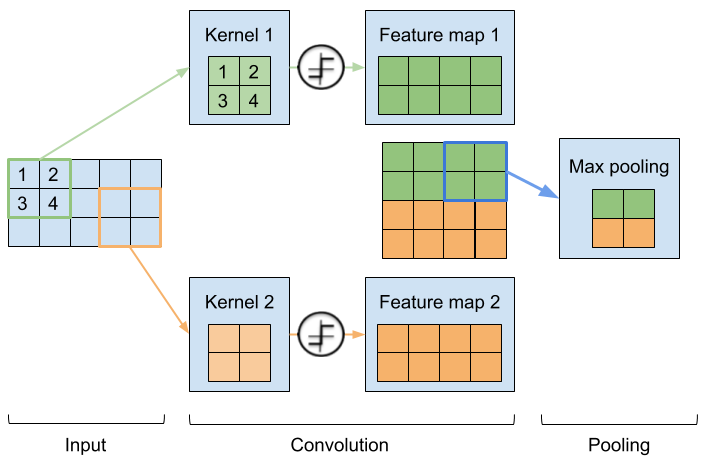
\includegraphics[width=12cm, height=7cm]{conv_net}
\caption[Illustration of convoltion and max pooling layers]{This figure illustrates the convoltion and pooling nodes of the \acrshort{conv_net}. In this example there is two kernels of size $2\times2$ with stride $1\times1$, which produce two feature maps. Each element in the feature maps are produced by taking the weighted sum of the kernel's input and passing the result through a non-linear activation function. Then the $2\times2$ max pooling is applied to each feature map to produce the final output.}
\label{fig:conv_net}
\end{figure}
\section{Deep \acrshort{conv_net}}

This section aims to motivate the improvement of the \acrshort{conv_net} by giving an overview of the varity of model based on it and the multitude of application domains.

\paragraph{Object detection:} Object detection is the field dedictated to the recognition of objects inside images. Over the recent years many models have been proposed to pull the error on the ImageNet data set \cite{imagenet_cvpr09} down. It started with the VGGNet \cite{DBLP:journals/corr/RussakovskyDSKSMHKKBBF14} and the AlexNet \cite{DBLP:journals/cacm/KrizhevskySH17}, which are simply deeper \acrshort{cnn}s. Then the GoogleNet \cite{DBLP:conf/cvpr/SzegedyLJSRAEVR15} introduced the Inception Module, which is able to extract multi-level features from the same input. Indeed, the Inception Module is using kernels of various size, i.e. $1\times1$, $3\times3$ and $5\times5$, to extract features from its inputs. Finally, the ResNet architechture \cite{DBLP:conf/cvpr/HeZRS16} introduced the idea of skip connections where some connections are directly linked to other layers much higer in the hierachy. The lastest archieved a top-5 error rate of 3.57\% on the ImageNet data set, which is composed of 1000 classes of objects.\newline

\noindent All those models shared the same building blocks (i.e. convolution and pooling layers) and have been successfully applied to the extraction of text from images, face recognition and scence understanding for autonomous vehicles.

\paragraph{Image segmentation:} Image segmentation is another important task in computer vision, which constists of a pixelwise binary prediction. The model is trained to predict one for all pixels that belongs to a class and zero otherwise. The state-of-the-art in image segmentation are architechture like UNet \cite{DBLP:conf/miccai/RonnebergerFB15} and LinkNet \cite{DBLP:conf/vcip/ChaurasiaC17}. Those architecture are composed of two parts, i.e. an encoder and a decoder. The encoder tranform the input image into a more compact representation that can then be unfold by the decoder to produce the final output.\newline

\noindent Needless to say that image segmentation models can be used to precisely determined the boundary of an object. Another advantage of this technique is that it can be used in collaboration with classical object detection to improve the accuracy of both the segmentation and the classification \cite{DBLP:conf/cvpr/KendallGC18}. The idea is that the encoder remains the same but several tasks are learned from it. The image segement task used the encoder as before while the object detection model used the features that it produce to to performs object detection.

\section{Conditional Principal Component Analysis}

The following explanation are based on the chapter 4 of \textcite{OReilly:2000:CEC:557205:chap4}. Hebbian learning is a biologically plausible and unsupervised learning thechnique based on the idea that neurons that trigger together must strentened their connection. The simplest learning rule in hevbbian learning as follow:

\begin{equation}
\Delta w_{ij} = \epsilon y_jx_i\ \ \ with\ \ \ y_j = \sum_{i}{x_i \times w_{ij}}
\end{equation}

\noindent where $\epsilon$ is the learning rate, $x_i$ is the i-th input, $y_j$ is the j-th output neuron, $w_{ij}$ is the i-th weight of the j-th neuron and $\Delta w_{ij}$ is the update for the weight $w_{ij}$. It can be show that this learning rule learned the first principal component of the data, but this technque has many limitations. First, the weights will become infinitly large as the neurons learn. This can be fix by using the Oja's rule, which normalize the weights update:

\begin{equation}
\Delta w_{ij} = \epsilon (x_iy_j - y_j^2w_{ij})
\end{equation}

\noindent Second, if many neurons are trained using the Oja's rule they will all learn the same component. This can be fix by using the Sanger's rule, which substract the information already explained by the first components:

\begin{equation}
\Delta w_{ij} = \epsilon (x_{stranger}y_j - y_j^2w_{ij})\ \ \ with\ \ \ x_{stranger} = x_i - \sum_{k = 1}^{j - 1}{y_kw_{ik}}
\end{equation}

\noindent Finally, all of the previous learning rules compute the principal component over all the data points. This become a problem when the data is very heterogeneous. Indeed, in the case of the figure \ref{fig:heterogeneous_data} (a) the component learned by such methods will correspond to the blue line, which does not represent well the shape of the data. In this case it is preferable to focus on only one of the two clusters as shows in figure \ref{fig:heterogeneous_data} (b) where the bottom-most cluster is ignored. This is the idea behind \acrshort{cpca}, indeed, in \acrshort{cpca} the neuron will relies on a conditioning function and learn only for learn for a subset of the data. The conditioning function used in this paper will be explained in the next section. The learning rule in \acrshort{cpca} is defined as follow:

\begin{equation}
\Delta w_{ij} = \epsilon y_j (x_i - w_{ij})
\end{equation}

\noindent This learning rule force each weigth $w_{ij}$ to tends to represent the probability of $x_i$ given that the neuron trigger, i.e. $w_{ij} = P(x_i = 1 | y_j = 1)$.

\begin{figure}[h]
\centering
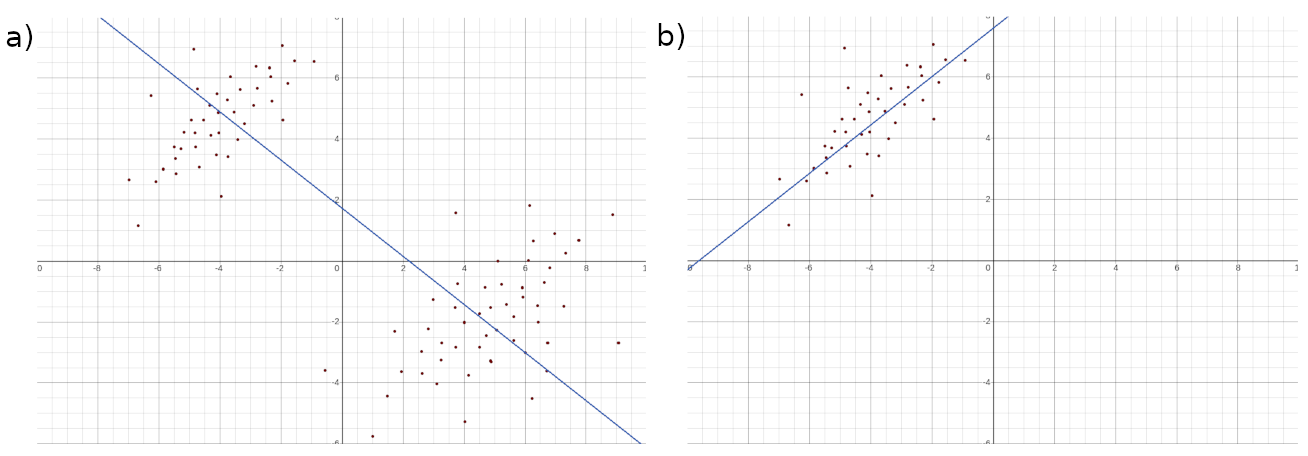
\includegraphics[width=15cm, height=5cm]{heterogeneous_data}
\caption[Illustration of heterogenous data points belonging to two clusters]{This figure shows heterogenous data points belonging to two clusters. On the right the first principal component is computed over all the data points. On the left the bottom-most cluster is ignored and the first principal component is computed only over the data points of the top-most cluster.}
\label{fig:heterogeneous_data}
\end{figure}

\section{K-Winner-Take-All} \label{sec:kwta}

The need for a conditioning function in \acrshort{cpca} have been highlighted in the previous section. This section presents the k-Winner-Take-All method that enable such conditioning. The k-Winner-Take-All aims to make only a subset of $k$ neurons to be active for each input. This can be archieved by either inhibiting all the neurons until only $k$ of them remaind active or by forcing the activation to $n - k$ neurons to zero, where $n$ is the total number of neuron in the node.\newline

Independently of the method chosen only the $k$ neurons which have the highest activation will remaind active. Those neurons are the ones whose weights fitted the best the input pattern. Since, the learning rule in \acrshort{cpca} is making the weights tends to $P(x_i = 1 | y_j = 1)$, then those neurons will fit the input even better. Finally, the last point of this section will be to explain how \acrshort{cpca} and \acrshort{kwta} are related to the figure \ref{fig:heterogeneous_data} (b). By now, it should be clear that \acrshort{kwta} will enable a neuron to ignore the bottom-most cluster if its weights does not fit it well. Additionally, the \acrshort{cpca} learning rule will allows the neuron to both fit the top-most cluster even better and learn a useful representation of the input for which it is reponsible.

\chapter{Mixing Model and Task Learning} \label{model_and_task_learning}

\section{Motivations}

The motivation behind a mixture of task and model learning, directly came from the advantages and disadvantages of each methods as explaned in chapter 6 of \textcite{OReilly:2000:CEC:557205}. For the sake of the example, let us consider the hebbian learning model, which belong to model learning algorithms. In hebbian learning, the units are learning local correlational structure of their inputs. This has the advantages of being reliable and autonomous. Indeed, the units are learning from the data (i.e. reliable) and does not depend on the activation of the neurons upper in the hiearachy (i.e. autonomous). However, this model suffer from its lake of vision and is unable to update its weights for serving a greater good such as solving a task, which is where the task learning algorithms come into play. The most popular task learning algorithm is the backpropagation algorithm. It has the advantages of being task-driven and cooperative. Indeed, the units are working together (i.e. cooperative) in order to solve a task (i.e. task-driven). On the other hand, the backpropagation is lazy as it stop learning when the task have been solved and the interdependency can slow down the learning as the gradients coming from defferent output units can balance each other out. To sum up, the model-based algorithm might enable the learning of reliable features and speed up the task learning by framing the model based on the incoming data.

\section{\acrlong{hcnn}}

\subsection{Mixing hebbian learning and backpropagation} \label{sec:mix_hebb_bp}

The idea of mixing hebbian learning and backpropagation have already been proposed by \textcite{OReilly:2000:CEC:557205}, where the authors shown how to combine backpropagation and hebbian learning such as:
\begin{equation}
\Delta_{weights} = \epsilon (ratio \times \Delta_{hebbian} + (1 - ratio) \times \Delta_{backpropagation})
\end{equation}
where $\Delta_{weights}$ is the final update of the weights, $\epsilon$ is the learning rate, $ratio$ is the amount of hebbian learning between zero and one, $\Delta_{hebbian}$ is hebbian update of the weights and $\Delta_{backpropagation}$ is backpropagation update of the weights. Finally, a reasonable value for the $ratio$ of hebbian is between $0.0005$ and $0.01$.

\subsection{\acrshort{cnn} with \acrshort{cpca} and \acrshort{kwta}}
The previous subsection explained how to mix hebbian learning and backpropagation. Also, this paragraph describe a new model, i.e. \acrshort{hcnn}, obtained by mixing a \acrshort{cnn} with \acrshort{cpca} and \acrshort{kwta}. The only layer modified in this model is the convolutional layer. As explained in section \ref{sec:mix_hebb_bp} the final weights update will be a mix between the \acrshort{cpca} and the backpropagation gradients. Additionaly, as explained in section \ref{sec:kwta} \acrshort{cpca} required a conditionning function to learn efficiently. This will be archieve using a \acrshort{kwta} competition between the neurons of the convolutional node. Figure \ref{fig:hcnn} shows the convolutional layer with \acrshort{cpca} and \acrshort{kwta}.

\begin{figure}[h]
\centering
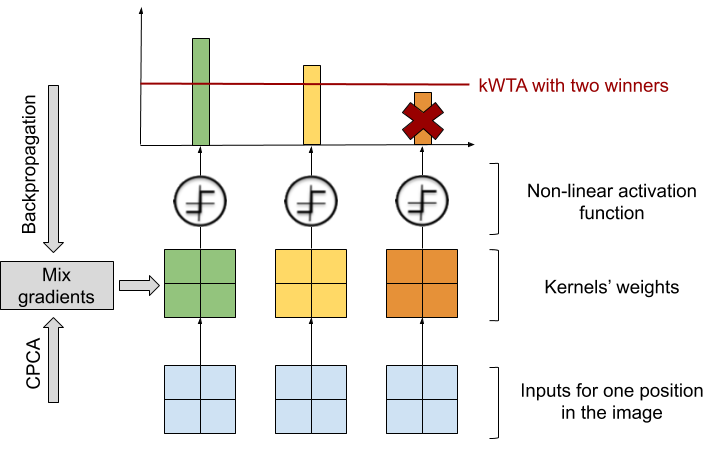
\includegraphics[width=15cm, height=10cm]{hcnn}
\caption[Illustration of the \acrlong{hcnn}]{This figure illustrate the convolutional layer of the \acrlong{hcnn}. The inputs are the same for all the kernel. The weights are used to computed the weighted sum of the inputs and the result is passed through a non-linear activation function. Then, the \acrshort{kwta} ensure that only two neurons win the competition and set the activation of the orange kernel to zero. Finally, the gradients of the backpropagation and \acrshort{cpca} are computed and mixed using the equation presented in section \ref{sec:mix_hebb_bp}.}
\label{fig:hcnn}
\end{figure}

\noindent In this model the \acrshort{kwta} competition allows to \acrshort{cpca} to learn more efficiently, i.e. conditioning function. It also brings more stability in the learning as only a subset of the neuron learn, i.e. change what they represent and react to. The \acrshort{cpca} on the other side add data-driven constraint on the way the weights are learned. This aims to avoid unrealistic pattern to be learned and can be seen as a regularization of the weights. Indeed, the equation of weights update, i.e. $\Delta w_{ij} = \epsilon y_j (x_i - w_{ij})$, shows that as the weights become large the difference between the data and weights, i.e. $x_i - w_{ij}$, become large and negative. This elegantly force the weights to remain small.

\chapter{Model implementation} \label{model_implementation}

This chapter discuss the implementation of the \acrshort{hcnn} model. The implementation have been written from scratch and aims to provide an easily extendable framework. The code have been tested properly using unit tests and code running on the GPU have been written in order to archieve harware acceleration. The code running on the \acrshort{cpu} have been written in Java and the code executed by the \acrshort{gpu} have been written using CUDA C.

\section{Data set}

In order to make the framework easily extendable, the code provide a data set interface, which allows to load the data by batch. Support for new data sets can easily be added by creating new classes that implement this interface. As soon as a new class have been implemented, the new data set become available using the data set factory. The following line of code create an instance of the mnist data set loading the example by batch of size twenty.

\begin{minted}[mathescape, linenos, numbersep=5pt,  frame=lines, framesep=2mm]{java}
DataSet dataSet = DataSetFactory.create("Mnist", 20);
\end{minted}

\noindent The data set interface is composed of six functions:

\begin{minted}[mathescape, linenos, numbersep=5pt,  frame=lines, framesep=2mm]{java}
    /**
     * Reload the data set.
     */
    public abstract void reload();

    /**
     * Reload the data set.
     * @param training true if training data set is required and false otherwise.
     */
    public abstract void reload(boolean training);

    /**
     * Check if there is a next batch.
     * @param training true if training data set is required and false otherwise.
     * @return true if there is a next batch and false otherwise.
     */
    public abstract boolean hasNextBatch(boolean training);

    /**
     * Select the next batch in the training set.
     * @param training true if training data set is required and false otherwise.
     */
    public abstract void nextBatch(boolean training);

    /**
     * Return the number of classes.
     * @return the number of classes.
     */
    public abstract int getNumberOfClasses();

    /**
     * Return the features corresponding to the current batch.
     * @param training true if training data set is required and false otherwise.
     * @return the features.
     */
    public abstract ArrayPtr getFeatures(boolean training);

    /**
     * Return the labels corresponding to the current batch.
     * @param training true if training data set is required and false otherwise.
     * @return the labels.
     */
    public abstract ArrayPtr getLabels(boolean training);
\end{minted}

\section{Nodes} \label{sec:nodes}

\subsection{Interface}

The code also provide a node interface, which can be used to add support for new nodes. As we will see in the next section, this generic interface allows to build complex graph of computation by linking the nodes with each other. The node interface is composed of six functions:

\begin{minted}[mathescape, linenos, numbersep=5pt, frame=lines, framesep=2mm]{java}
    /**
     * Compute the node activation.
     * @param training the mode (training vs testing).
     * @param x is the input.
     * @return the activation.
     */
    public abstract ArrayPtr activation(boolean training, ArrayPtr... x);

    /**
     * Update the weights.
     * @param lr the learning rate.
     * @param gradients the back propagation gradients from the upper nodes.
     * @return the gradients with respect to the node's inputs.
     */
    public abstract ArrayPtr[] update(double lr, ArrayPtr... gradients);

    /**
     * Save the node to the file.
     * @param kryo the kryo object.
     * @param output the kryo output.
     */
    public abstract void save(Kryo kryo, Output output);

    /**
     * Load weights from file.
     * @param kryo the kryo object.
     * @param input the kryo input.
     * @return this.
     */
    public abstract Node loadWeights(Kryo kryo, Input input);

    /**
     * Load node from file.
     * @param kryo the kryo object.
     * @param input the kryo input.
     * @return this.
     */
    public abstract Node load(Kryo kryo, Input input);

    /**
     * Display the node on the standard output.
     */
    public abstract void print();
\end{minted}

\noindent The framework currently support the following nodes:
\begin{itemize}
	\item \textbf{Dense} which is a fully connected node;
	\item \textbf{Conv2d} which is a 2D convolutional node supporting \acrshort{cpca} and  \acrshort{kwta};
	\item \textbf{MaxPooling2d} which is a 2D max pooling node;
	\item \textbf{Flaten} which transform a multi-dimensional data into a flat representation;
	\item \textbf{Merge2d} which merge many inputs into a single output;
	\item \textbf{Activation} which apply various activation functions such as sigmoid and softmax;
	\item \textbf{Add} which perform an element wise addition;
	\item \textbf{AvgPooling2d} which is a 2D mean pooling node;
	\item \textbf{Identity} which forward the input, i.e. identity node;
	\item \textbf{KWTA2d} which perform 2d K-Winners-Takes-All competition;
	\item \textbf{Pad2d} which apply padding on 2d data.
\end{itemize}

\noindent The following subsections focus on explaining the backpropagation of the most important nodes.

\subsection{Flaten}

The flatten node simply reshape the data for example if the input is a $3\times3$ matrix the node flatten it as a vector of size 9. During the backpropagation the node will receive the derivative of the error function with respect to the each output neuron, i.e. a vector of size 9. This node does not have any weights and will just return the derivative of the error function with respect to the input, i.e. the vector of size 9 is reshaped and a $3\times3$ matrix is returned.

\subsection{MaxPooling2d}

The max pooling is quite similar to the flatten node, because it does not have any weights to update. During the forward pass the node keep in memory the mask that will be used to backpropagate the gradients. This mask has the same shape as the input and contains a one if the cell was the highest value of the pooling kernel and zero otherwise. Assuming a $2\times2$ max pooling node and a $4\times4$ input matrix the node will output a $2\times2$ matrix and keep in memory a $4\times4$ mask matrix. During the backward pass the node received a $2\times2$ matrix containing the derivative of the error function with respect to the each output neuron. The gradient are backpropagate by using the mask, indeed, each pooling kernel of the mask is multiplied by the corresponding gradient as sown in figure \ref{fig:max_pooling_bp}.

\begin{figure}[h]
\centering
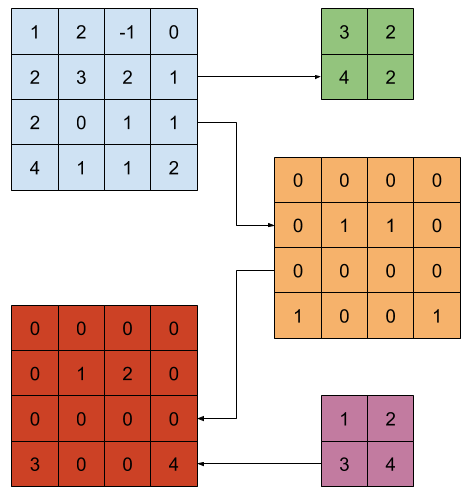
\includegraphics[width=4.5cm, height=5cm]{max_pooling_bp}
\caption[Backropagation in max pooling layer]{This figure illustrate the forward and backward pass of the max pooling node. The blue matrix is the input data, the green is the node output and the orange one is the mask corresponding to the input. Finally, the purple matrix is the matrix containing the derivative with respect to the output of the neurons and the red one contains the derivative with respect to the input.}
\label{fig:max_pooling_bp}
\end{figure}

\subsection{Dense}

The dense node is more interresting, because of two reasons. First, the node has weights to update, which required to compute the derivative with respect to the weights in addition to the derivative with respect to the inputs. Second, the node has an activation function that makes the problem a bit more difficult. The first notion required to correctly explained the backpropagation in a dense node is known as the chain rule, which is defined by:

\begin{equation}
\frac{\delta z}{\delta x} = \frac{\delta z}{\delta y} \times \frac{\delta y}{\delta x}
\end{equation}

\noindent where $z$ is a function of $y$ and $y$ a function of $x$. In a dense node each neuron $j$ compute its net input $z_j$ as a weighted sum of its inputs such as:

\begin{equation}
z_j = \sum_{i}{x_i \times w_{ij}}
\end{equation}

\noindent where $z_j$ is the net input of the j-th neuron, $x_i$ is the i-th input and $w_{ij}$ is the i-th weight of the j-th neuron. The net input is then pass through an activation function $\sigma$ such as:

\begin{equation}
y_j = \sigma(z_j)
\end{equation}

\noindent where $y_j$ is the activation of the j-th neuron. During the backpropagation the node needs to determined the derivative of the error function with respect to the weights and the inputs. The chain rules give us the following for the weights:

\begin{equation}
\frac{\delta e}{\delta w_{ij}} = \frac{\delta e}{\delta y_j} \times \frac{\delta y_j}{\delta z_j} \times \frac{\delta z_j}{\delta w_{ij}}
\end{equation}

\noindent where $\frac{\delta e}{\delta y_j}$ is the derivative of the error function with respect to the activation of the output of the j-th neuron. The derivative of the error function with respect to the input is a bit more complexe, because it required to sum over all the output neurons of the node.

\begin{equation}
\frac{\delta e}{\delta x_{i}} = \sum_{j} \frac{\delta e}{\delta y_j} \times \frac{\delta y_j}{\delta z_j} \times \frac{\delta z_j}{\delta x_i}
\end{equation}

\noindent The derivative of the error function with respect to the weights will be used to update the weights and the derivative with respect to the inputs will be used as the derivative with respect to the output of the previous node.

\subsection{Conv2d} \label{sec:conv2d}

This section has two objectives. First, it aims to explain the backpropagation in convolutional nodes. Second, it aims to explains how to compute the \acrshort{cpca} gradients. Let's start with the computation of the backpropagation gradients for both the weights and the inputs. The only difference for the computation of the weights' gradients is the appearance of a sum over all the positions of the image where the weights have been applied:

\begin{equation} \label{eq:dwc2d}
\frac{\delta e}{\delta w_{ij}} = \sum_{k} \frac{\delta e}{\delta y_{jk}} \times \frac{\delta y_{jk}}{\delta z_{jk}} \times \frac{\delta z_{jk}}{\delta w_{ijk}}
\end{equation}

\noindent where $y_{jk}$ is the activation of the j-th neuron at the position $k$, $z_{jk}$ is the net input of the j-th neuron at the position $k$ and $w_{ijk}$ is the i-th weigth of the j-th neuron at position $k$. Note that the weights are the same for all positions $k$, but $\frac{\delta z_{jk}}{\delta w_{ijk}}$ change as $k$ change. Indeed, this derivative is actually $x_{ijk}$, i.e. the input corresponding to the $w_{ij}$ when applied at position $k$. Figure \ref{k_weights_vs_inputs} (b) aims to clarify the meaning of the position $k$. A comparable summation appear for the derivative with respect to the inputs:

\begin{equation}
\frac{\delta e}{\delta x_{i}} = \sum_{l} \sum_{j} \frac{\delta e}{\delta y_{jl}} \times \frac{\delta y_{jl}}{\delta z_{jl}} \times \frac{\delta z_{jl}}{\delta x_{il}}
\end{equation}

\noindent where $x_{il}$ is the input whose derivative is being computed; as explained the $l$ index is only relevant for the weights. Indeed, $x_{il}$ is the same input for all the value of $l$, but $\frac{\delta z_{jl}}{\delta x_{il}}$ change as $l$ change. Indeed, this derivative is actually $w_{lj}$, i.e. the weight corresponding to the input $x_{i}$ at position $l$. Figure \ref{k_weights_vs_inputs} (b) aims to clarify the meaning of the position $l$.

\begin{figure}[h]
\centering
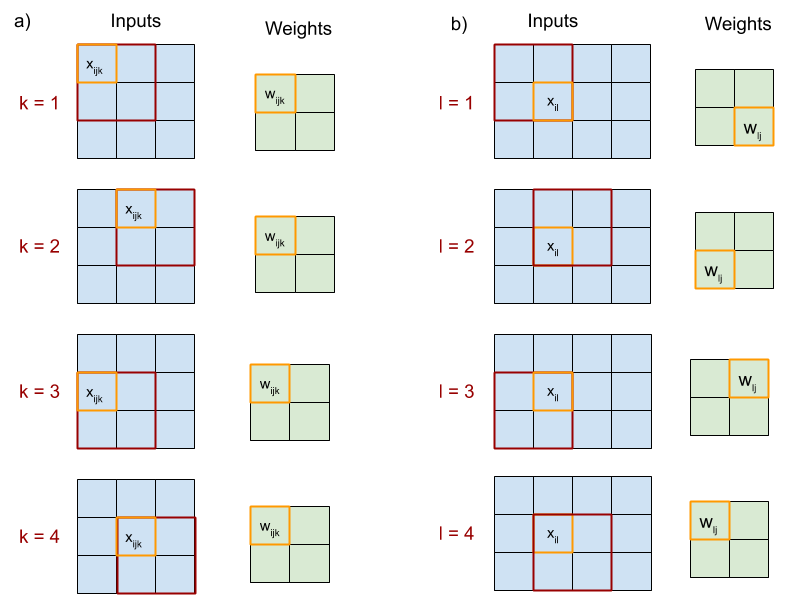
\includegraphics[width=10cm, height=8cm]{k_weights_vs_inputs}
\caption[Backpropagation in convoluational layers: meaning of indexes]{This figure aims to clarify the meaning of the indexes $k$ and $l$. (a) The index $k$ iterate through all the positions of the input image taking steps whose size are defined by the strides of the node. (b) The index $l$ iterate through all the positions where the kernel contains the input $x_i$.}
\label{k_weights_vs_inputs}
\end{figure}

\noindent Let's now focus on the second goal of this subsection, i.e. explaining how to compute the \acrshort{cpca} gradients. The idea is to iterate through all the positions of the input image taking steps whose size are defined by the strides of the node and to compute the mean of the \acrshort{cpca} learning rule such as:

\begin{equation}
\Delta w_{ij} = \frac{\epsilon}{|K|} \sum_{k} y_{jk}(x_{ik} - w_{ij})
\end{equation}

\noindent where $w_{ij}$ is the i-th weights of the j-th neuron, $\epsilon$ is the learning rate, $|K|$ is the number of position in the image, $y_{jk}$ is the output of the neuron $j$ at position $k$ and $x_{ik}$ is the i-th input at position $k$. The constant $|K|$ can even be absorbed by the learning rate $\epsilon$ giving raise to an even simpler equation:

\begin{equation}
\Delta w_{ij} = \epsilon \sum_{k} y_{jk}(x_{ik} - w_{ij})
\end{equation}

\section{Computational Graphs}

\subsection{Graph}

This subsection aims to explains how to build a graph of computation and how the backpropagation have been implemented. The first step to create a graph is to create the nodes and set their inputs to create the graph's connectivity. It can be done as follow:

\begin{minted}[mathescape, linenos, numbersep=5pt,  frame=lines, framesep=2mm]{java}
// Create three nodes.
Node conv2d = NodesFactory.create("Conv2d");
Node flatten = NodesFactory.create("Flatten");
Node output = NodesFactory.create("Dense");

// Create the connectivity.
flatten.setInputs(conv2d);
output.setInputs(flatten);
\end{minted}

\noindent Then, the graph can be created from the graph's configuration. The only thing required for the creation of the configuration is to set the graph's outputs.

\begin{minted}[mathescape, linenos, numbersep=5pt,  frame=lines, framesep=2mm]{java}
// Create the graph's configuration.
GraphConf conf = new GraphConf().setOutputs(output);

// Create the graph according to the configuration.
Graph graph = new Graph(conf);
\end{minted}

\noindent Let's now focus on the backpropagation of the gradients through the graph, which is archieved by a recursive function presented in the pseudo code below:

\begin{minted}[mathescape, linenos, numbersep=5pt,  frame=lines, framesep=2mm]{java}
Create a map between each node and its corresponding array of gradients.
// There are as many gradients as parents of the node.
// The gradients are initially missing, i.e. null.
Compute the gradient with respect to the output of the graph.
// The gradients of the output node are now available in the map.
Start recursion // i.e. backpropagation(graph's output, map)

void backpropagation(node, map)
    if all the gradients of the node are available // i.e. non-null
        Compute the gradient with respect to the output of the node
        // i.e. nodeGradient = map[node].sumGradientsElementWise()
        Compute the gradient with respect to the output of the children
        // i.e. childrenGradients = node.update(nodeGradient)
        // The gradients of the node's children are now available in the map.
        for all child in node.children
            backpropagation(child, map)
\end{minted}

\begin{figure}[h]
\centering
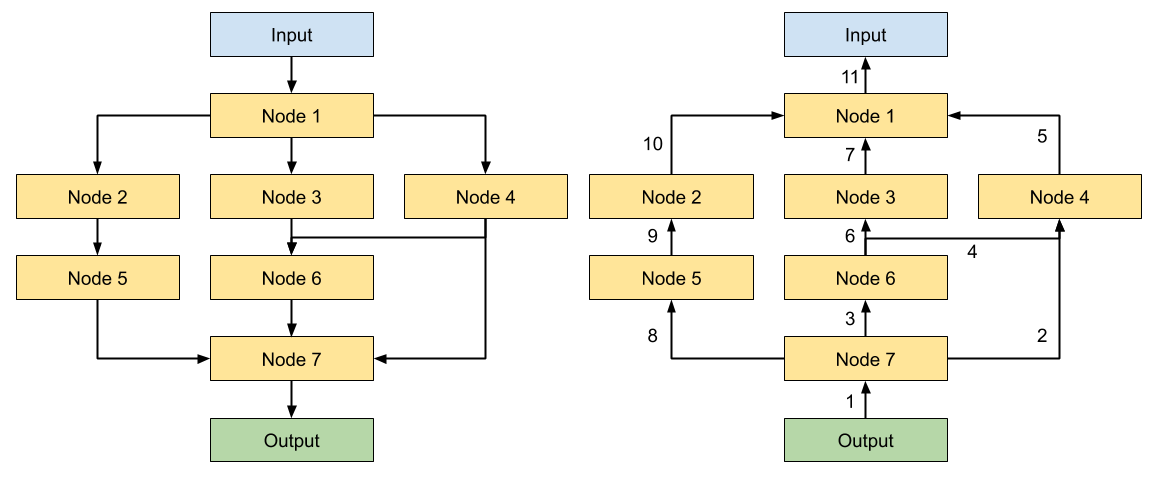
\includegraphics[width=10cm, height=5cm]{graph_bp}
\caption[Backpropagation of the gradients in a graph of computation]{This figure shows how the gradients are backpropagated through the graph. On the left, the arrows represent the flow of data during the forward pass, i.e. graph connectivity. On the right, the arrows correspond to the computation of the gradients with respect to the nodes' inputs. The order in which the gradients are computed during the reccuresive process is shown by the number associate to each arrow.}
\end{figure}

\subsection{Neural Network}

The neural network class simplify the creation of sequential neural network, i.e. any stack of nodes. Also, it provides the function \mintinline{java}{addLayer} that add a node on the top of the stack. Its role is to build the underlying graph of computation.

\begin{figure}[h]
\centering
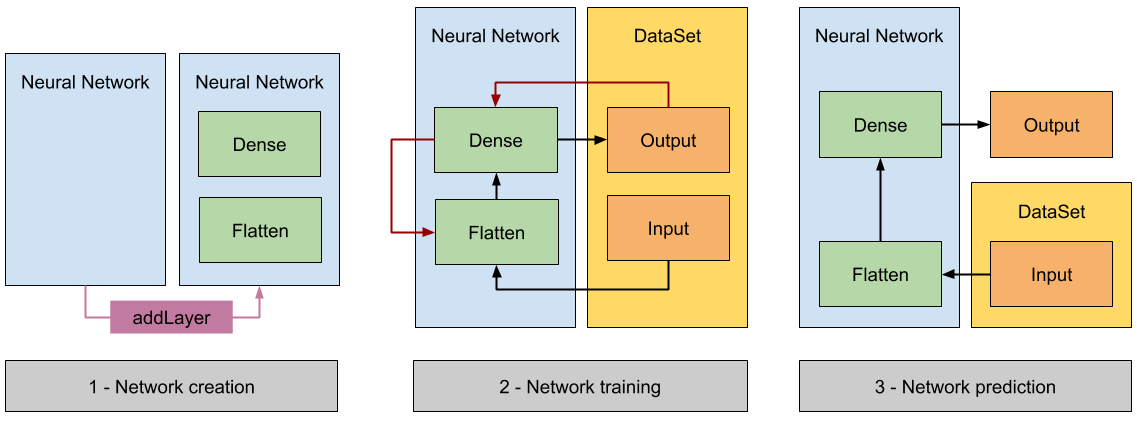
\includegraphics[width=15cm, height=5cm]{neural_network}
\caption[Interactions between neural network, nodes and data set]{This figure shows how the neural network, the nodes and the data set interact with each other. The first use case shows nodes being added to the stack. The second shows the training of the network where the black arrows are calls to the \mintinline{java}{activation} function and the red arrows the calls to the \mintinline{java}{update} function. Finally, the third use case shows the prediction process using the same color code.}
\end{figure}
\newpage

\section{Zoo}

\subsection{AlexNet}

The zoo provide an implementation of many state-of-the-art models. The AlexNet is a deep ConvNet presented by Alex Krizhevsky in 2012. This 
model greatly reduced the top-5 error on the ImageNet data set, i.e. from $26\%$ to $15.3\%$. In the fundation paper the model have been trained during six days on two GTX 580. The implementation available in the zoo does not support multi-GPUs training. Table \ref{table:alexnet} and Figure \ref{fig:alexnet} show the details of the AlexNet architechture. 

\begin{table}[h!]\label{table:alexnet}
\centering
\begin{tabular}{  c  c  }
Layer type & Layer details\\
\hline
Conv2d & 96 filters of $11\times11$ and strides of $4\times4$ \\
MaxPooling2d & pooling kernel of $2\times2$ \\
Conv2d & 256 filters of $5\times5$ and strides of $1\times1$ \\
MaxPooling2d & pooling kernel of $2\times2$ \\
Conv2d & 384 filters of $3\times3$ and strides of $1\times1$ \\
Conv2d & 384 filters of $3\times3$ and strides of $1\times1$ \\
Conv2d & 256 filters of $3\times3$ and strides of $1\times1$ \\
MaxPooling2d & pooling kernel of $2\times2$ \\
Flatten & \\
Dense & 4096 output units \\
Dense & 4096 output units \\
Dense & 1000 output units and softmax activation
\end{tabular}
\caption[AlexNet architecture]{This table shows layers of the AlexNet architechture.}
\end{table}

\begin{figure}[h]\label{fig:alexnet}
\centering
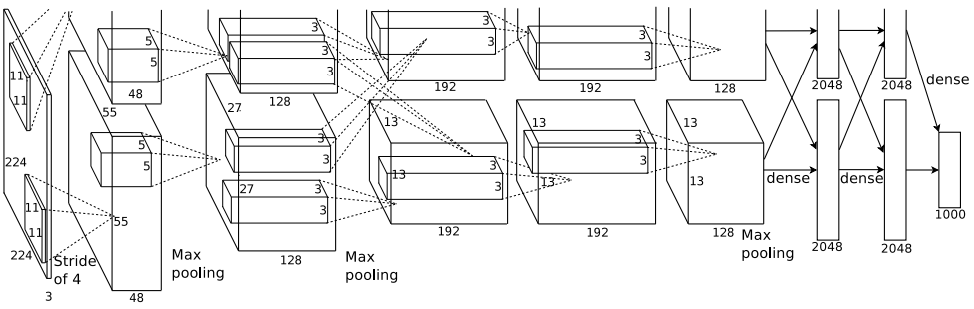
\includegraphics[width=15cm, height=5cm]{alexnet}
\caption[AlexNet architecture]{This figure come from the AlexNet paper \cite{DBLP:journals/cacm/KrizhevskySH17}. It illustrates the AlexNet architecture and explicitly showing the delineation of responsibilities between the two GPUs. One GPU runs the layer-parts at the top of the figure while the other runs the layer-parts at the bottom. The GPUs communicate only at certain layers.}
\end{figure}

\newpage
\subsection{VGG}

Two years later Simonyan and Zisserman developed the VGG, which pull the top-5 error down to $8.0\%$. Figure \ref{fig:alexnet} show the details of the VGG architechtures. The framework implement the configuration A, B, D and E.

\begin{figure}[h]\label{fig:vgg}
\centering
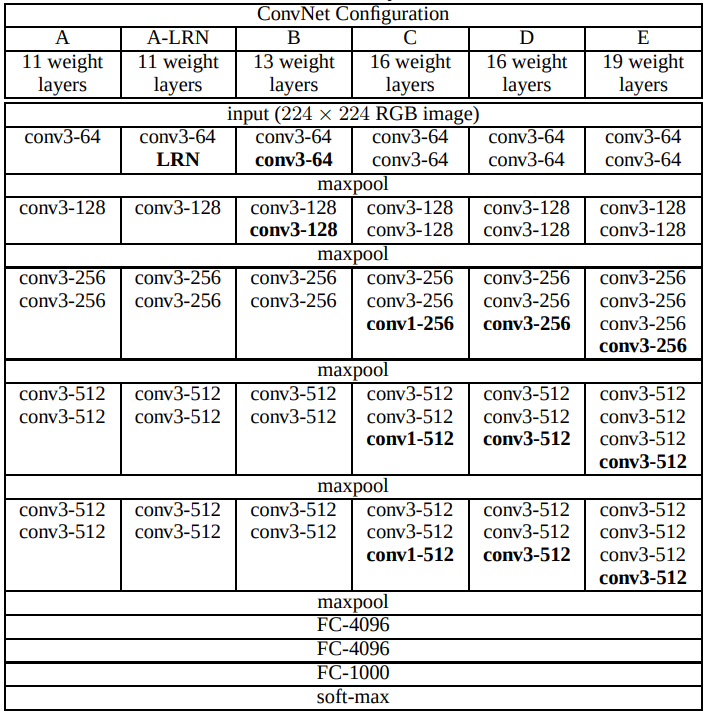
\includegraphics[width=11cm, height=12cm]{vgg}
\caption[VGG architecture]{This figure come from the VGG paper \cite{DBLP:journals/corr/RussakovskyDSKSMHKKBBF14}. It illustrates the VGG11, VGG13, VGG16 and VGG19 architecture. The ReLU activation function is not shown for brevity. The convolutional layer parameters are denoted as "$conv<receptive\ field\ size>-<number\ of\ channels>$".}
\end{figure}

\newpage
\subsection{ResNet}

In 2015, Kaiming He and al. introduced the idea of skip connections and achieve a top-5 error rate of $3.57\%$. In the fundation paper three kind of skip connections have been proposed. The simplest one perform an identity mapping. The second perform a zero padding, when the number of filters of the input does not match the number of filters of the output. The last one perform a linear projection using a $1\times1$ convolution layer. The result of the skip connection is then added to the output of the last layer of the residual block. The final step of the residual block is to apply the relu activation function. The framework support the three kind of skip connections and provide an implementation all the ResNet architectures, i.e. $ResNet[18|34|50|101|152]$.

\begin{figure}[h]\label{fig:resblock}
\centering
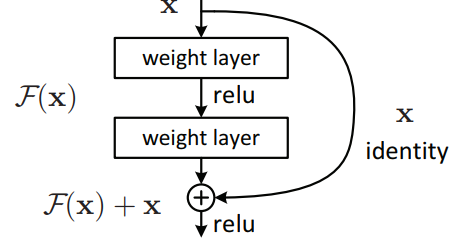
\includegraphics[width=8cm, height=4cm]{resblock}
\caption[Residual block]{This figure come from the ResNet paper \cite{DBLP:conf/cvpr/HeZRS16}. It illustrates the residual building block.}
\end{figure}

\begin{figure}[h]\label{fig:resnet}
\centering
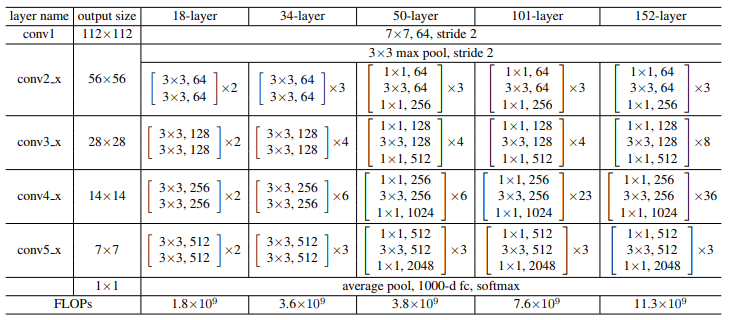
\includegraphics[width=11cm, height=5cm]{resnet}
\caption[ResNet architecture]{This figure come from the ResNet paper \cite{DBLP:conf/cvpr/HeZRS16}. It illustrates the ResNet18, ResNet34, ResNet50, ResNet101 and ResNet152 architecture.}
\end{figure}

\newpage
\section{Unit testing}

The unit tests have been written using JUnit 5 and ensure that the code is working properly. The following code shows one of the 145 unit tests written:

\begin{minted}[mathescape, linenos, numbersep=5pt, frame=lines, framesep=2mm]{java}
class OperationTest {
    @Test
    void sum() {
        // Create the operation and the input.
        OperationInterface op = OpsFactory.create("Operation", "cpu");
        ArrayPtr x = create(new float[][]{{1, 2}, {2, 1}});
        // Check the validity of the sum, i.e. 1 + 2 + 2 + 1 = 6.
        assertEquals(6, op.sum(x));
    }
}
\end{minted}

\noindent Since, this framework is about backpropagation it is important to ensure that the gradients are correctly computed. The unit tests are implementing a technique named numerical gradient checking to check the correctness of the gradients. The key is to compute an approximation of the derivative with respect to a variable such as:
\begin{equation}
g(x) = \frac{df(x)}{dx} = \lim_{k\to0} \frac{f(x + k) - f(x - k)}{2k}
\end{equation}
where $g$ is the derivative, $f$ is the function and $x$ is variable.
Figure \ref{fig:gradient_checking} illustrates the idea behind this method for the function: $f(x) = x^{2}$. A neural network can be see as a parameterized function $f$ that transform some imput $x$ into an output $f(x, \theta)$ based on the weigths $\theta$. In this context the variable can either be $x$ or $\theta$. The approximation of the derivative is then compared with the actual value computed by the neural network.

\begin{figure}[h]
\centering
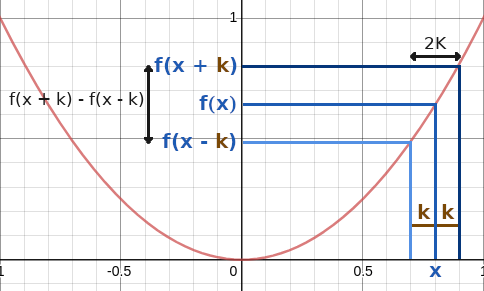
\includegraphics[width=8cm, height=5cm]{gradient_checking}
\caption[Illustration of the numerical gradient checking method]{Illustration of the numerical gradient checking method.}
\label{fig:gradient_checking}
\end{figure}

\section{\acrlong{gpu}}

\subsection{Core concepts} \label{sec:core_concepts}

The \acrshort{gpu} was initially designed for graphics application where the need for parallelization is huge due to the large number of pixels to process. In order to provide such parallelization \acrshort{gpu} are generally composed of hundreds if not thousands of cores. Each core can then processes data in parallel. Originally, the API available to run code on GPU was OpenGL and DirectX, which was specialize in graphics computation. It only in November 2006 that NVIDIA unveiled the GeForce 8800 GTX built with the CUDA architechture enabling guneral-purpose computation.
\\

\begin{figure}[h]
\centering
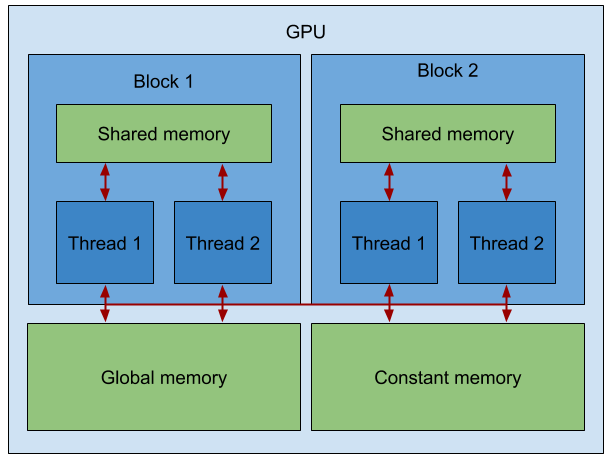
\includegraphics[width=10cm, height=6cm]{gpu_architecture}
\caption[Illustration of the GPU architecture]{Illustration of the GPU architecture. The red arrows link the threads to the memory they can access. The gloabal memory is the basic memory accessible from every threads. The constant memory is similar to the gloabal memory, but is accessible in read-only. Finally, the shared memory is shared amoung threads of the same block. Also, the need to syncronize the threads appears for any application that needs to reduce the shared memory, e.g. computing the sum of all the elements. This can be archieve by calling the function \mintinline{cuda}{__syncthreads()} to ensure that all threads finished their job.}
\label{fig:gpu_architecture}
\end{figure}

\noindent Figure \ref{fig:gpu_architecture} shows the GPU architecture. The following aims to explain how to use the CUDA API. The first thing to understand is the difference between the host and the device. The host refer to the CPU and the device refer to the GPU. A kernel is a function which run on the device and can be called from the host. A kernel does not return any value and must be annotate with the qualifier \mintinline{cuda}{__global__}, which tell the NVIDIA compiler that the function is actually a kernel.

\begin{minted}[mathescape, linenos, numbersep=5pt,  frame=lines, framesep=2mm]{cuda}
__global__ void kernel(int parameter, float *result) { ... }
\end{minted}

\noindent Another important qualifier is \mintinline{cuda}{__device__}, which tell the NVIDIA compiler that the function will be executed on the device. A device function can be call from any kernel or device function.

\begin{minted}[mathescape, linenos, numbersep=5pt,  frame=lines, framesep=2mm]{cuda}
__device__ float device_function(int parameter) { ... }
\end{minted}

\noindent The last thing to understand is how the threads are organized. Indeed, threads are arranged into blocks and blocks are packed to form the grid. Blocks and threads can have indexes in up to three dimension. The figure \ref{fig:grid} shows a visual representation of the grid.
\\

\begin{figure}[h]
\centering
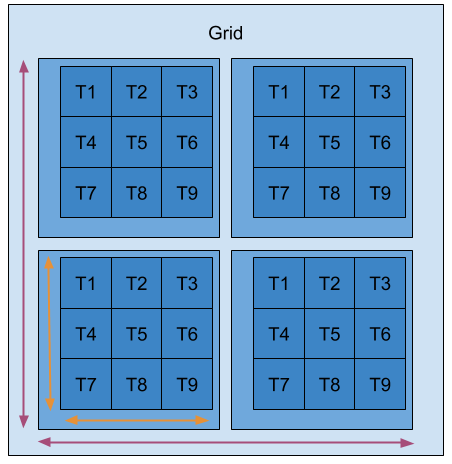
\includegraphics[width=6cm, height=5.5cm]{grid}
\caption[Illustration of the GPU grid]{An example grid where both blocks and threads have 2D indexes. The purple arrows show the blocks dimensions and the orange arrows show the threads dimensions.}
\label{fig:grid}
\end{figure}

\noindent Finally, the indexes of the thread and block being processed are available in the kernel through the variables: \mintinline{cuda}{threadIdx.x}, \mintinline{cuda}{threadIdx.y}, \mintinline{cuda}{threadIdx.z}, \mintinline{cuda}{blockIdx.x}, \mintinline{cuda}{blockIdx.y} and \mintinline{cuda}{blockIdx.z}. Also, the number of threads and blocks are available in the kernel through the variables: \mintinline{cuda}{blockDim.x}, \mintinline{cuda}{blockDim.y}, \mintinline{cuda}{blockDim.z}, \mintinline{cuda}{gridDim.x}, \mintinline{cuda}{gridDim.y} and \mintinline{cuda}{gridDim.z}.

\subsection{Application to neural networks}

Section \ref{sec:core_concepts} has presented all the main concepts of CUDA C, the following describes how it have been used to speed up the framework. First, it is worth noting that some computer does not have \acrshort{gpu}. Also, it is useful to provide a factory that instanciate either the \acrshort{cpu} or the \acrshort{gpu} implementation depending on the hardware available in the computer. The following line load the correct implementation for the $Conv2d$ node:

\begin{minted}[mathescape, linenos, numbersep=5pt,  frame=lines, framesep=2mm]{java}
Node conv_2d = NodesFactory.create("Conv2d");
\end{minted}

\noindent \textcite{DBLP:journals/tjs/BritoFCSWMF16} show that \acrshort{gpu}s can be successfully used to speed up artificial neural networks. Even if the framemork has a \acrshort{gpu} implementation for all nodes presented in \ref{sec:nodes}. The following paragraphs focus on the backward pass in 2D convolutional node. Indeed, it is one of the most challenging to understand and a clear explanation will provide great insight for using \acrshort{gpu} to speed up neural networks. This kernel is using all the blocks and threads dimensions, i.e. all the following indexes are used: \mintinline{cuda}{threadIdx.x}, \mintinline{cuda}{threadIdx.y}, \mintinline{cuda}{threadIdx.z}, \mintinline{cuda}{blockIdx.x}, \mintinline{cuda}{blockIdx.y} and \mintinline{cuda}{blockIdx.z}. The block indexes are used to go through all the weights that are stored in a 4D array, i.e. the first dimension corresponds to the number of neurons in the layer, the second to the number of input channels, and finally, the third and fourth to the kernel's width and height respectively. Because there is only three blocks indexes (i.e. $x$, $y$ and $z$), the first one is used to go through the two first dimensions. As explained in section \ref{sec:conv2d} the computation of the derivatative with repect to the weights required to sum the gradients over all positions $k$, cf equation \ref{eq:dwc2d}. As previously explained, each block is responsible to compute the derivative with respect to one weight, i.e. all weights are computed in parrallel. Moreover, the threads of each block proccess several part of the images at the same time. The threads' $x$ index iterate through all the images of the batch being processed, the $y$ index trough all the vertical positions and $z$ index trough all the horizontal positions. The shared memory is used by each thread to store the sum of all the positions it is responsible. Then, the \mintinline{cuda}{__syncthreads()} function is called to synchronize all the threads. Finally, the first thread of each block sum the elements of the shared memory and place the result in the output buffer. The figure \ref{fig:conv2d_backpropagation} illustrate this process for a batch of two images.

\begin{figure}[h]
\centering
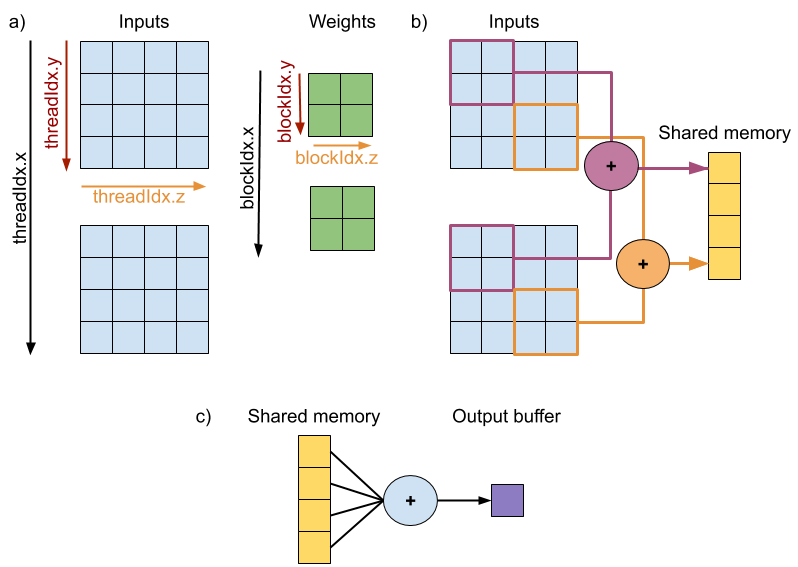
\includegraphics[width=9cm, height=7cm]{conv2d_backpropagation}
\caption[Illustration of the GPU-enabled backpropagation in convolutional layer]{This figure illustrate the GPU-enabled backpropagation in the convolutional layer. For the sake of simplicity this figure assumes two images with only one channel and two kernels of size $2\times2$. a) shows the meaning of the blocks and threads indexes. b) shows how the summation over all the positions is performed in parallel. This assume a $2\times2$ stride and a $1\times2\times2$ grid of blocks. The first thread, i.e. purple, is responsible for the top right positions within each images. The last thread, i.e. orange, is responsible for the bottom left positions within each images. c) shows the sum of the elements in the shared memory preformed by the first thread of each block after the call to the \mintinline{cuda}{__syncthreads()} function.}
\label{fig:conv2d_backpropagation}
\end{figure}

\subsection{Optimization of data movement}

This subsection explains an optimization which enabled the framework to run three time faster. It aims to highlight the amount of time lost when the data is moved back and forth between the CPU and the GPU. Indeed, the first implementation of the framework was copying the data from the CPU to the GPU before each kernel call. After the call, the result was copied backward, i.e. from the GPU to the CPU.
\\

\noindent The new implementation has introduced the $ArrayPtr$ class. This class aims to abstract the location of the data. Because the $ArrayPtr$ can be passed directly from one node to the other, the data can stay on the device. The time that was needed to move the data back and forth between the host and the device is saved.

\chapter{Results and Analysis} \label{result_and_analysis}

\section{\acrshort{gpu} vs \acrshort{cpu}}

\subsection{Hardware specifications}

This subsection aims to give the hardware specifications of the CPU and GPU used for the benchmarks. The GPU implementations have been tested on a Pascal Tesla P100, which belongs to the Pascal generation and deliver up to 10.6 TFLOPS of single precision (FP32) performance. The CPU implementation have been tested on a Intel Xeon E5520 CPUs running at 2.27GHz, which has 4 cores, i.e. 8 threads.

\subsection{Layers}

In this section the CPU and GPU implementation of six layers are presented. The speed of each layer have been evaluated for 100, 1000 and 10000 iterations. One iteration correspond to both the forward and the backward pass. The iteration is performed on ten MNIST images, which correspond to an array of $10\times1\times28\times28$ for the $MaxPooling2d$ and $Conv2d$ layers as well as an array of $10\times784$ for the $Dense$ layer. Each experiment have been ran ten times and the tables below show the mean of execution time and the standard deviation (STD).
\newline
\newline
\noindent The first interresting thing to look at is that some layers are more suited to the GPU implementation. Indeed, the GPU-enabled Conv2d and MaxPooling layers are up to 5990 times faster that their CPU counterparts. On the other hand, the GPU implementation of the Dense layer is only 12 times faster. This is due to the the property of the problem being solved efficently by the GPU. The first kind of layers require a huge amount of  computation that can be computed in parallele, i.e. at different position of the image. The Dense layer is more difficult to parallelize, because each neuron to need to compute a weighted sum of its inputs. This weighted sum can be seen as a global statistic difficult to parallelize. It also require threads synchronization, which leading to a lost of performance.
\newline
\newline
\noindent Second, the table \ref{table:CNN_vs_HCNN} shows the additional time required to compute the CPCA gradients and kWTA activation. This extra-time seems to grow with the number of iterations. The convolutional layer is up to 1.5 times faster than its conterpart with CPCA and kWTA.

\begin{table}[h!]
\centering
\begin{tabular}{ c c c c c c }
Iterations & Device time (ms) & Device STD & Host time (ms) & Host STD & Speed up\\
\hline
100   & 295  & 46.58 & 171996   & 4380   & 583 \\
1000  & 931  & 61.17 & 1651739  & 49192  & 1774 \\
10000 & 5967 & 96.09 & 16600000 & 622521 & 2782
\end{tabular}
\caption[Speed benchmark: Conv2d layer]{Speed comparison between CPU and GPU implementation of the Conv2d layer.}
\end{table}

\begin{table}[h!]
\centering
\begin{tabular}{ c c c c c c }
Iterations & Device time (ms) & Device STD & Host time (ms) & Host STD & Speed up\\
\hline
100   & 289  & 53    & 191000   & 5074   & 661 \\
1000  & 954  & 40.05 & 1830000  & 19134  & 1918 \\
10000 & 6298 & 94.26 & 18100000 & 435109 & 2874
\end{tabular}
\caption[Speed benchmark: Conv2d layer with kWTA]{This table shows the speed benchmark between the CPU and the GPU implementation of the Conv2d layer with kWTA.}
\end{table}

\begin{table}[h!]
\centering
\begin{tabular}{ c c c c c c }
Iterations & Device time (ms) & Device STD & Host time (ms) & Host STD & Speed up\\
\hline
100   & 359  & 42.37  & 183000   & 4587   & 510 \\
1000  & 1270 & 60.58  & 1730000  & 38130  & 1362 \\
10000 & 8562 & 108.50 & 17100000 & 216927 & 1997
\end{tabular}
\caption[Speed benchmark: Conv2d layer with CPCA]{This table shows the speed benchmark between the CPU and the GPU implementation of the Conv2d layer with CPCA.}
\end{table}

\begin{table}[h!]
\centering
\begin{tabular}{ c c c c c c }
Iterations & Device time (ms) & Device STD & Host time (ms) & Host STD & Speed up\\
\hline
100   & 339  & 41.05  & 198000   & 3324   & 584 \\
1000  & 1241 & 64.08  & 1880000  & 32474  & 1515 \\
10000 & 8954 & 119.40 & 19000000 & 319616 & 2122
\end{tabular}
\caption[Speed benchmark: Conv2d layer with CPCA and kWTA]{This table shows the speed benchmark between the CPU and the GPU implementation of the Conv2d layer with CPCA and kWTA.}
\end{table}

\begin{table}[h!]
\centering
\begin{tabular}{ c c c c c c }
Iterations & Device time (ms) & Device STD & Host time (ms) & Host STD & Speed up\\
\hline
100   & 115  & 11.80 & 1360  & 294.70 & 12 \\
1000  & 302  & 15.72 & 3090  & 409.92 & 10 \\
10000 & 1969 & 24.89 & 13100 & 612.96 & 7
\end{tabular}
\caption[Speed benchmark: Dense layer]{Speed comparison between CPU and GPU implementation of the Dense layer.}
\end{table}

\begin{table}[h!]
\centering
\begin{tabular}{ c c c c c c }
Iterations & Device time (ms) & Device STD & Host time (ms) & Host STD & Speed up\\
\hline
100   & 12  & 2.72  & 26600   & 585   & 2217 \\
1000  & 58  & 10.58  & 238000  & 3296  & 4103 \\
10000 & 394 & 20.07 & 2360000 & 37037 & 5990
\end{tabular}
\caption[Speed benchmark: MaxPooling2d layer]{Speed comparison between CPU and GPU implementation of the MaxPooling2d layer.}
\end{table}

\begin{table}[!htb]
\centering
\begin{tabular}{ c | c c | c c | c }
Iterations & Conv2d (ms) & STD & Hebbian Conv2d (ms) & STD & Speed up\\
\hline
100   & 295  & 46.58 & 339  & 41.05  & 1.1492 \\
1000  & 931  & 61.17 & 1241 & 64.08  & 1.3330 \\
10000 & 5967 & 96.09 & 8954 & 119.40 & 1.5006
\end{tabular}
\caption[Speed benchmark: Computational cost of CPCA and kWTA]{This table shows the computational cost of CPCA and kWTA in the GPU implementation of the Conv2d layer. The third line can be read as follows: for 10000 iterations the Conv2D is 1.5 times faster than its conterpart with CPCA and kWTA.}\label{table:CNN_vs_HCNN}
\end{table}
\FloatBarrier

\subsection{Networks}

In this section the CPU and GPU implementation of four networks are presented. All network are composed of four layers:

\begin{itemize}
	\item \textbf{Conv2d} with 8 filters of $2\times2$, strides of $2\times2$ and a relu activation function;
	\item \textbf{MaxPooling2d} with $2\times2$ pooling kernel;
	\item \textbf{Flaten};
	\item \textbf{Dense} with 10 output units.
\end{itemize}

\noindent The difference between the four networks is that the first does not use neither CPCA nor kWTA, the second use kWTA, the third use CPCA and the fourth use both CPCA and kWTA. Each network have been tested on 1 and 3 epochs. One epoch is defined by the training of the network over the entire MNIST dataset. Each experiment have been ran ten times and the tables below show the mean of execution time and the standard deviation (STD).

\begin{table}[h!]
\centering
\begin{tabular}{ c c c c c c }
Epochs & Device time (ms) & Device STD & Host time (ms) & Host STD & Speed up\\
\hline
1 & 5908  & 91.59  & 13600000 & 245293 & 2302 \\
3 & 13777 & 152.16 & 42100000 & 357999 & 3056
\end{tabular}
\caption[Speed benchmark: Conv2d network]{This table shows the benchmark between the CPU and the GPU implementation of the Conv2d network.}
\end{table}

\begin{table}[h!]
\centering
\begin{tabular}{ c c c c c c }
Epochs & Device time (ms) & Device STD & Host time (ms) & Host STD & Speed up\\
\hline
1 & 5933  & 62.66  & 14200000 & 281201 & 2393 \\
3 & 14126 & 134.05 & 44100000 & 703370 & 3122
\end{tabular}
\caption[Speed benchmark: Conv2d network with kWTA]{This table shows the benchmark between the CPU and the GPU implementation of the Conv2d with kWTA network.}
\end{table}

\begin{table}[h!]
\centering
\begin{tabular}{ c c c c c c }
Epochs & Device time (ms) & Device STD & Host time (ms) & Host STD & Speed up\\
\hline
1 & 7150  & 246.93 & 15900000 & 662694  & 2224 \\
3 & 17522 & 438.07 & 49100000 & 2540731 & 2802
\end{tabular}
\caption[Speed benchmark: Conv2d network with CPCA]{This table shows the benchmark between the CPU and the GPU implementation of the Conv2d with CPCA network.}
\end{table}

\begin{table}[h!]
\centering
\begin{tabular}{ c c c c c c }
Epochs & Device time (ms) & Device STD & Host time (ms) & Host STD & Speed up\\
\hline
1 & 7364  & 210.29 & 14900000 & 400573  & 2023 \\
3 & 17924 & 318.31 & 44700000 & 1301869 & 2494
\end{tabular}
\caption[Speed benchmark: Conv2d network with CPCA and kWTA]{This table shows the benchmark between the CPU and the GPU implementation of the Conv2d with kWTA and CPCA network.}
\end{table}
\newpage

\section{\acrshort{hcnn} vs \acrshort{cnn}}

Learning speed

%TODO

\chapter{Framework limitations} \label{framework_limitation}

This chapter aims to explains the current limitations of the framework and their implications. The first limitation is that the graph does not support multiple inputs and outputs. This become a problem to implement models such as the GoogleNet, which require three time the same output as shown in figure \ref{fig:googlenet}.

\begin{figure}[h]
\centering
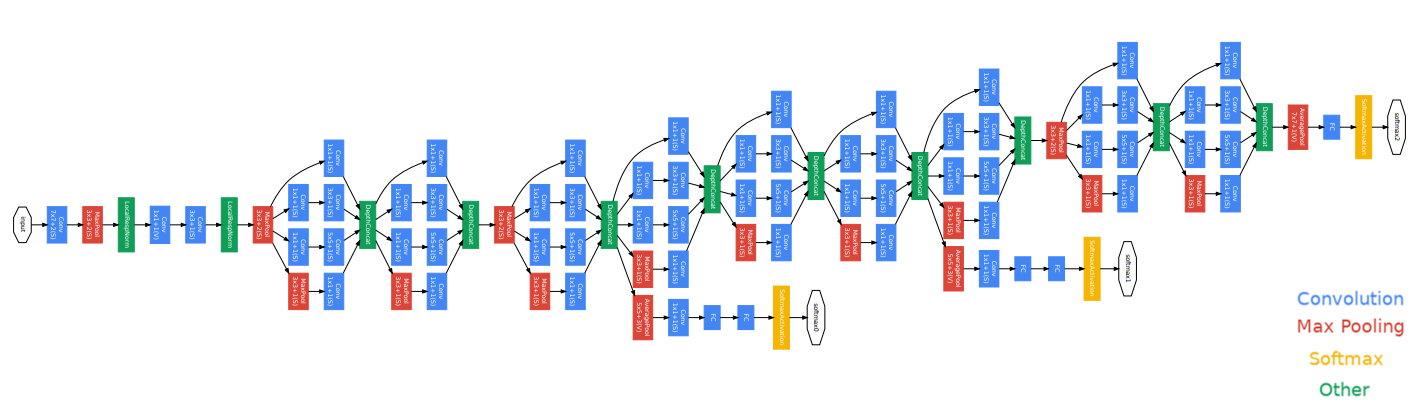
\includegraphics[width=16cm, height=5cm]{googlenet}
\caption[GoogleNet architecture]{This figure come from the GoogleNet paper \cite{DBLP:conf/cvpr/SzegedyLJSRAEVR15} and illustrate the GoogleNet architecture. Each softmax function is linked to the label to predict, i.e. multi-output graph of computation.}
\label{fig:googlenet}
\end{figure}
\noindent The max and mean pooling layers does not support overlapping. Indeed, the framework only support pooling where the strides have the same size as the pooling kernel. This introduce slight differences between the original implementation of the AlexNet and the zoo implementation.
\newline
\newline
\noindent Local response normalisation, weights decay and dropout are also missing from the VGG implmentation available in the zoo. The UNet and LinkNet used in image segmentation cannot be implemented, because the deconvolutional layer is still unavailable.
\newline
\newline
\noindent Finally, additional work is needed in order to allow very big models such as the ResNet152 to run properly. Indeed, this kind of model reach the limit of memory available on the device and additional transfers of data must be implemented to avoid that the program crash.

\chapter{Conclusion and Future Research} \label{conclusion}

%TODO conclude

%TODO future direction
Probalistic model

\printbibliography

\end{document}
